\chapter{Aporte práctico}

En el capítulo 3 se presentaron algunas técnicas y herramientas que sirven para el aprendizaje colaborativo; No obstante, para objetivos de esta tesis, se requiere una herramienta que integre ciertas características de las que ya poseen las mencionadas en el capítulo anterior. Ver Tabla \ref{tab:herramientasAC}.\\
 
El sistema que se pretende desarrollar estará basado en el proceso para la elaboración de sesiones de clase usando la técnica de Jigsaw con la particularidad de que en esta ocación la generación de grupos expertos no será siempre de forma aleatoria sino que también se podrá realizar basándose en información del estudiante respecto a su estilo de aprendizaje y preferencias sobre el tema a desarrollar y los miembros posibles para su grupo. Esta última característica no forma parte de la estructura tradicional de la técnica de Jigsaw y la técnica de Pair Research como se puede ver en la tabla \ref{tab:tecnicasAC}.\\

El sistema a desarrollar también tendrá la particularidad de que permitirá a los estudiantes trabajar de forma colaborativa en la elaboración de archivos de código fuente, los cuales serán producto de las respuestas que dichos alumnos darán a los problemas que les plantee el profesor durante la sesión de clase jigsaw. Por ende, para lograr este objetivo y tener dicha funcionalidad en el sistema se usará los frameworks y APIs descritas en el capítulo anterior. Ver tabla \ref{tab:frameworks}.

\section{Las mejores prácticas de RUP}
EL Proceso Unificado Rational(RUP) es un proceso de ingeniería de software que provee un enfoque para la asignación de tareas y responsabilidades durante el desarrollo de un software. Tiene como objetivo asegurar la producción de un producto software de alta calidad que satisfaga los requerimientos de los usuarios finales dentro de un tiempo y presupuesto establecido \cite{rup_ibm_2014}. Ver figura \ref{fig:rup}\\

\begin{figure}[!h]
  \centering
  % Requires \usepackage{graphicx}
  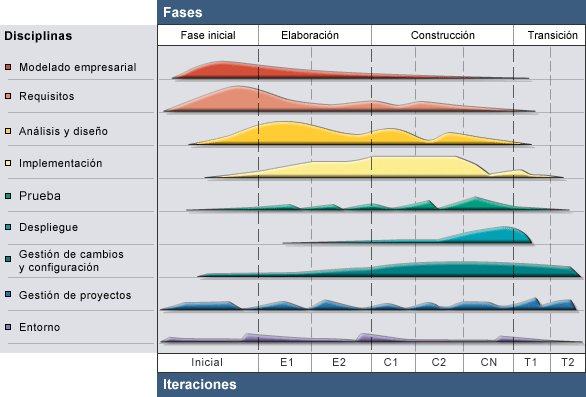
\includegraphics[scale=0.7]{figuras/rup.jpg}\\
  \caption[RUP]{Proceso de desarrollo de software - RUP \protect\cite{rup_small}}\label{fig:rup}
\end{figure}

Así mismo, RUP también es una guía para usar de manera efectiva el Lenguaje Unificado de Modelado (UML) que no es más que un lenguaje estándar que permite comunicar claramente los requerimientos, arquitecturas y diseños \cite{rup_ibm_2014}.\\

Es por ello que el desarrollo del sistema propuesto por esta tesis estará guiado por la buenas prácticas de RUP, estableciéndose iteraciones semanales en las cuales se irá desarrollando cada una de las fases en las que RUP divide el ciclo de desarrollo de software: Inicio, Elaboración, Construcción y Transición. Los artefactos que serán entregados durante el proceso de desarrollo del sistema web de tiempo real para el aprendizaje colaborativo propuesto en esta tesis se mencionan en la Tabla \ref{tab:artefactos_rup}. Dichos artefactos se encuentran agrupados según la disciplina a la que pertenecen.

\begin{longtable}{|L{6cm}|L{9cm}|}
\caption{Artefactos del proceso de desarrollo}
\label{tab:artefactos_rup}\\
    \hline
    DISCIPLINA RUP & ARTEFACTO \\
    \hline
    \multirow{2}{*}{Requisitos} & $\bullet$ Modelo de caso de uso\\
    \hhline{~~} & $\bullet$ Especificaciones suplementarias\\
    \hline
    \multirow{5}{*}{Análisis y diseño} & $\bullet$ Modelo de análisis\\
    \hhline{~~} & $\bullet$ Modelo de datos\\
    \hhline{~~} & $\bullet$ Prototipo de interfaz de usuario\\
    \hhline{~~} & $\bullet$ Documento de arquitectura de software\\
    \hhline{~~} & $\bullet$ Mapa de navegación\\
    \hline
    \multirow{2}{*}{Implementación} & $\bullet$ Código fuente\\
    \hhline{~~} & $\bullet$ Sistema web desplegado\\
    \hline
    \multirow{2}{*}{Prueba} & $\bullet$ Casos de prueba\\
    \hhline{~~} & $\bullet$ Resultados de prueba\\
    \hline
\end{longtable}

\clearpage
Para el desarrollo del sistema web, se seguirá el siguiente cronograma, el mismo que se está orientado a seguir las actividades y tareas que plantea RUP. Se indica también las fechas en las cuales se estará aplicando el sistema al caso de estudio.

\begin{figure}[!h]
  \centering
  % Requires \usepackage{graphicx}
  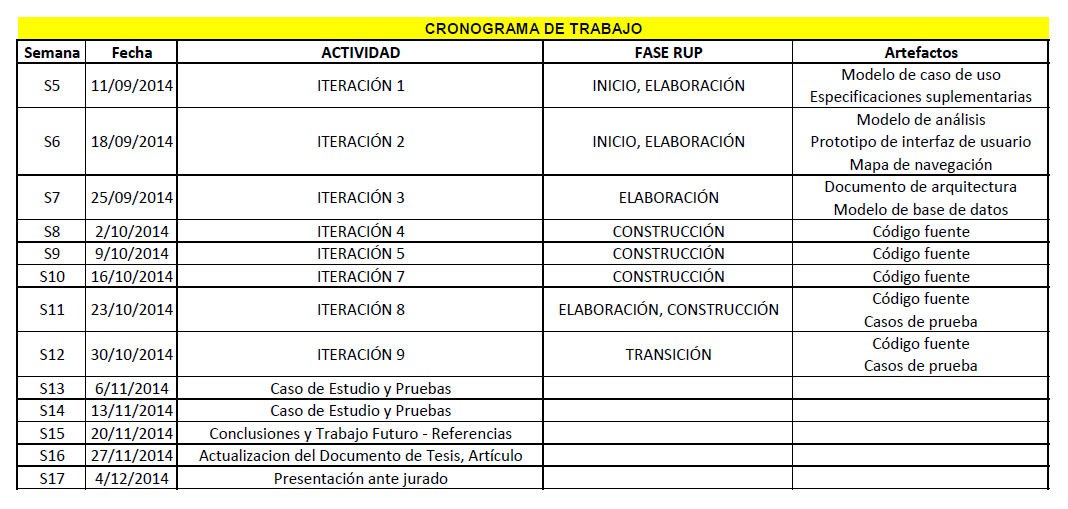
\includegraphics[scale=0.5]{figuras/cronograma.png}\\
  \caption[CRONOGRAMA]{Cronograma de trabajo}\label{fig:cronograma}
\end{figure}

%\begin{longtable}{|L{2.5cm}|L{2cm}|L{5cm}|L{5cm}|}
%\caption{CRONOGRAMA}
%\label{tab:cronograma}\\
%    \hline
%    ITERACIÓN & FECHA & FASE RUP & ARTEFACTO \\
%    \hline
%    1 &	11-09-2014	&	INICIO, ELABORACIÓN	& Modelo de caso de uso, Especificaciones suplementarias\\
%
%    \hline
%\end{longtable}

\section{Implementación de un sistema web de tiempo real para el aprendizaje colaborativo}

\section{} 